\chapter{基于弱监督注意力的多人姿态估计方法}
\label{cha:method}

\section{概述}
\label{sec:methodoverview}
%   This part intends to state the overall idea
本方法使用基于残差网络\footnote{残差网络,简称ResNet, 全称Residual Network}与特征金字塔网络\footnote{特征金字塔网络,简称FPN, 全程Feature Pyramid Network}结构的网络框架作为特征提取的骨架,为模型提供各个尺度的特征图。在特征提取部分之后,网络可以分为目标检测与姿态估计和融合回归两个步骤。在目标检测与姿态估计过程中,网络预测出目标的边界框,粗略的关键点预测和实例分割结果。而在融合回归部分,网络会接受从目标检测与姿态估计阶段产生的结果并将它们一同以一定的方式互相交汇并一起回归。而且,在融合回归的过程中,网络采取了多阶段的堆叠和中继监督的策略来共同精炼关键点与实例分割的结果。这种结构是受到CPM\cite{wei2016convolutional}的启发而设计的。同时,为了有效地融合实例分割与姿态估计的结果,网络使用了注意力机制,使其根据实例分割的生成注意力关注网络对应的区域,从而达到方法最初设计的目的,也就是解决多人检测下姿态遮挡的问题。同时,考虑到姿态估计的信息对实例分割也有促进作用,我们设计了双流的网络结构让模型在每个阶段都能同时预测分割结果和姿态估计结果,并送入下一阶段继续优化。网络的整体结果如图\ref{fig:Overall}

%	ROI Extraction
%	key-point & Mask Prdiction
%		Stage One's Prediction
网络通过特征提取器$E$得到图像$I$来自网络各个尺度的特征$F=\{f_1, f_2, ..., f_5\}$。这些特征被兴趣区域对齐层\footnote{兴趣区域对齐层,简称RoI Align Layer, 全称Region of Interest Align Layer}通过双线性插值的方法调整到了同样的尺寸。每个图像中只有来自特定尺度$k$的特征图$f_k$被选中并被输入至接下来的目标检测与姿态估计部分。这个被选中的特征被分别送入了目标检测分支$D$与姿态估计分支$P$,分别得到了实例分割结果$S_1=\{s_1^1, s_1^2, ..., s_1^n\}$与姿态估计结果$K_1=\{k_1^1, k_2^1, ..., k_1^n\}$。这些中间结果会被输入到融合优化阶段进行多阶段的回归。

\begin{figure*}[htbp]	
	\centering
	\includegraphics[scale=0.4]{network.eps}
	\caption{网络整体结构}
	\label{fig:Overall}
\end{figure*}

%		Stage 2+'s Prediction
如图\ref{fig:RefineNet}所示,在融合优化阶段的第$t(t>2)$阶段,单个优化模块接收来自特征提取器$E$的特征$f_k$、在阶段$t-1$中得到的姿态估计结果$K_{t-1}$与实例分割结果$S_{t-1}$。整个网络有主要设计亮点可以归纳为三点。第一是我们引入了注意力机制让网络关注具体的区域,我们设计了\textit{Attention Converter}来让生成一个合适的注意力与特征图融合,最后得到关键点预测结果$K_t$。第二,网络还会根据姿态估计的中间结果,也就是一些更偏向于得到关键点预测的特征,生成实例分割的结果。这让网络会根据来自姿态估计的信息修正实例分割的结果。最后,由\textit{Attention Converter}生成的注意力还会与从姿态估计那一支生成的中间结果融合,最终生成的实例分割的优化结果$S_t$。因此,整个优化模块$R$可以被抽象为形如公式\eqref{def:refinenet}的函数。


\begin{equation}
\label{def:refinenet}
M_t, K_t = R(M_{t-1}, K_{t-1})
\end{equation}

%   This part is to describe why we use a hybrid multi-stage arch
%	1. mask and key-point detection is associated
%	2. In crowd, the heatmap is not robust to predict
本方法使用了多阶段、利用弱监督约束的注意力的结构,同时优化实例分割与姿态估计的结果。首先多阶段与中继监督这两个设计可以让网络获得更大的感受野,让网络能够充分学习关键点之间的关系\cite{wei2016convolutional}。其次,由于实例分割和姿态估计是联系紧密的两个任务, 正如本文\ref{sec:generalmotivation}中提到的,实例分割与姿态估计能够相互优化,并且有相当大的相关性。所以这样设计的结构主要是希望能够同时优化姿态估计与实例分割结果。通过引入注意力以及弱监督这种较宽松约束下的可学习参数,网络能够更加适应数据中的不同表现。这让网络在一些实例分割无法正确引导关键点检测的情况下, 仍然能够生成较为正确的注意力引导关键点的检测与人体骨架的重建。

\begin{figure*}[htbp]	
	\centering
	\includegraphics[scale=0.65]{RefineNet.pdf}
	\caption{融合优化模块具体设计}
	\label{fig:RefineNet}
\end{figure*}

\section{目标检测与姿态估计}
\label{sec:detectionstage}
%	Structure description
%	1. Hybrid arch of maskrcnn & cpm
本文在特征提取部分使用了101层的残差网络与特征金字塔网络来生成不同尺度的特征图供检测部分使用。正如Mask R-CNN\cite{He2017Mask}中使用的结构,本文也设计了并行的区域建议网络,在经过回归分支后从不同尺度的特征图上得到来自不同尺度的边界框。这些尺度不同的边界框会根据其来源送入专为特征金字塔网络设计的兴趣区域对齐层,根据公式选定对应的层数来裁剪并对齐特征图\cite{Lin2016Feature}。这样裁剪下来的特征图具有相对平衡的感受野:小尺寸物体有较小的感受野大小,同时大尺寸物体会获得更大的感受野大小。

检测部分是由两个并行的分支组成的。实例分割与姿态估计分支分别使用裁剪好的特征得到粗略的实例分割结果与姿态估计结果。分割分支的网络结构使用了四层卷积核大小为3像素的卷积层,和一层步长为2,卷积核大小为2的空洞卷积层。同样的,姿态估计分支使用了五层卷积核大小为3的卷积层,最终的输出被两层1x1卷积调整至关键点外加背景个通道,以得到每个关键点的热力图。


%   Training strategy description
%	Section 1
在检测部分的监督过程中,由于我们将网络设计为能够完成两个任务的并行的分支,所以该部分的损失函数设计就表现为两个损失函数加和的形式,如公式\eqref{detection_loss}所示。首先我们需要对目标位置检测进行监督,所以我们就借鉴区域卷积神经网络\cite{Girshick_2014_CVPR}中损失函数设计思路,使用交叉熵来计算预测标签与真实标签之间的距离。同样的,如Mask R-CNN\cite{He2017Mask}中的损失函数设计,交叉熵也被用来监督实例分割。公式\eqref{bbox_mask_loss}描述目标检测与实例分割的损失函数设计。姿态估计分支的损失函数被定义为均方差的形式,如公式\eqref{coarse_key-point_loss}所示。

\begin{equation}
%	section 1 loss
\label{detection_loss}
L_{detection} = L_{bbox\&mask_{reg}} + L_{key-point_{reg}}
\end{equation}      
\begin{equation}
%	bbox & mask regression loss
\label{bbox_mask_loss}
L_{bbox\&mask_{reg}} = -\sum_{c \in C}{\hat{p_c} \log{p_c^{*}}}  -\sum_{c \in C}{\hat{m_c} \log{m_c^{*}}}
\end{equation}
\begin{equation}
%	coarse mask regression loss
\label{coarse_key-point_loss}
L_{key-point_{reg}} = -\sum_{i \in I}\sum_{k \in K}{\left\| \hat{k_i} - {k_i}^{*} \right\|_2}
\end{equation}


\section{融合优化}
\label{sec:refine}
\subsection{网络结构}
\label{subsec:architecture}
%	TODO: more detailed content to discuss the net structure in refine section
%	1. What the network looks like
%	2. Why we propose the network like this? (need to be explain by experiments)
%		a) training process (featured points)
%			(i)		loss penalty calculation
%		b) inference process 
%			(i)		attention-like instance segmentation
%Size of reception field is crucial to the refine section, as the key-point branch need them to avoiding the wrong decision in 
融合优化阶段由数个完全一样的优化模块组成,每个模块可以被抽象地定义为公式\eqref{def:refinenet}。
% TODO: bookmark in chapter 03

The refine section is divided into 5 seperated stages, and each part can be denoted as equation\eqref{def:refinenet}, to be more in detail, the network can be defined as below:
\begin{equation}
c = C({f}\otimes{K_{t-1}})
\end{equation}
\begin{equation}
a = A(f\otimes{M_{t-1}})
\end{equation}
\begin{equation}
K_t = H_k(c\odot a)
\end{equation}
\begin{equation}
M_t = H_m(F(c) \oplus a)
\end{equation}
第一份拷贝会首先与来自阶段$t-1$的姿态结果$K_{t-1}$进行合并,并一同被送入一组\textit{Shared Convolution Layers}中。第二份拷贝同样会与上一阶段的实例分割结果$S_{t-1}$进行合并,并被输入至\textit{Attention Converter}中。经过\textit{Shared Convolution Layers}的特征图会与\textit{Attention Converter}中$\sigma$门生成的注意力热图相乘。最终输出对关键点估计优化的结果$K_t$。同时\textit{Shared Convolution Layers}的特征图的另一份拷贝在经过两层卷积层后,会与\textit{Attention Converter}中$\tanh$门的输出相加,输出对实例分割的优化结果$S_t$。

where $\otimes$ refers to concatenating operation, $\odot$ for bit-wise multiply, and $\oplus$ is for bit-wise add operation. $M_t$ and $K_T$ denote the mask and key-point prediction from stage $t$. The feature map is denoted as $f$, and $a$ is for attention, $c$ is for the output from the shared convolution layers. In notations for modules, $C$ is for shared convolution layers, $A$ is for attention converter, and $F$ is for the fusion module. $H_k$ is for the key-point head, and the $H_m$ is for mask head.\\
It is common to generate attention using a given feature from last stage, and we suppose that the instance segmentation prediction, still can be treated as a strong cue to the soft attention. Therefore, our method proposed a attention converter to digest features and mask prediction from last stage to generate proper attention to the network.\\
However, the attention may be incompatible for a multi-staged architecture to supervise. Hence, a single layered mask head is designed here to adjust the dimension to the binary mask, which makes it easier to define losses to the attention. In another hand, like other the traditional multi-tasking networks, our method also employs a separated head which accepts features from a shared convolution to use the common priors which are used by the key-point prediction. To hybrid those two idea in the design of networks, we proposed the refine stage which is shown in Fig.\ref{fig:RefineNet}.\\

\subsection{损失函数定义}
\label{subsec:lossfunctions}
%	Section 2 Training
%	key-point Loss
%	Why Applying masks after 1x1 conv?
%	1.	explicitly define loss with mask & key-points
%	2.	simply enhance response of the heatmap
%		rather than enhance the result
%			--> This will give more responses
%	TODO: quote attention paper to prove it
Training strategy in section 2 is divided into two parts: key-point branch loss and instance segmentation loss. Loss in section 2 can be defined as a summing function from the second stage to the last \eqref{total_refine_loss}, where $\alpha$ is 0.05.

%	TODO: fit the <Attention is all you need> thread into this section
Training key-point branch is similar to the process in section 1. We define MSE loss to measure errors between ground truth and prediction. But what is different in section 2 is that the key-point predictions are affected by the instance mask implicitly, as we multiply them with those masks in a bit-wise fashion before 1x1 convolution layers. The 1x1 convolution layers will not change the size of reception field, therefore the operation we perform here are nearly the same as multiplying after the network. But with those trainable parameters in 1x1 convolution layers, the network will need no explicit definition of any masks in loss function of the key-point branch and also can strengthen the response at relative positions on feature maps. This is intended to avoid multiplying zeros on the result in key-point branch, which causes failure on supervising both key-point prediction and instance segmentation with one loss. The loss function in key-point branch $L_{k_t}$ where $t>1$ is defined as \eqref{refine_key-point_loss}. 

%	Total Refine Loss
\begin{equation}
\label{total_refine_loss}
L_{refine} = \sum_{t=2}^{T}{L_{k_t} + \alpha L_{m_t}}
\end{equation}

%	Refine key-point Loss
\begin{equation}
\label{refine_key-point_loss}
L_{k_{t}} = -\sum_{i \in I}\sum_{j \in J}{\parallel \hat{k_i} - {k_i}^{*} \parallel_2}
\end{equation}

%	Instance segmentation supervision
%	Localization loss
%		smoothed L1
%			attention-like
%	TODO: More attention paper quotations
Supervising mask branch is a more complicated process, because we want to train the network in order to complete the losing part where the detection section failed to infer. Therefore we consider to calculate both localization error and overlap penalty \eqref{mask_loss} for stage $t$ where $t>1$. We set the $beta$ in equation\eqref{mask_loss} to 0.2. The localization error is defined as \eqref{mask_loc_loss}. Instead applying a cross entropy loss here, we introduce smoothed L1 loss here, as the network use instance segmentation as attention.

%	Mask Loss
%	Semi supervision
\begin{equation}
\label{mask_loss}
L_{m_t}=L_{loc_t} - \beta L_{ins\ penalty_t}
\end{equation}

\begin{equation}
\label{mask_loc_loss}
L_{loc}^t =  \sum_{p \in P} Smooth_{L1}( H^{p}_{gt} - H^{p}_{pred} )
\end{equation}

\subsection{训练策略}
\label{subsec:trainingstrategy}
%	TODO: Training Strategy
%	Training Setups
%		learning rate
%		optimizer
%		separated trained ( sec 1 -> sec 2)
We use a two-stage separated training strategy. In the first stage, we train the joint branch only at learning rate of 4e-4 (all stages) for 60 epochs, with the epoch size of 1000 and the exponential learning rate decay (0.333 every 20 epoch). In the second stage, we train the whole refine branch with the total Loss, which equals to refine joint loss plus refine mask loss multiply by ten, with the base lr 1e-4 with exponential decay of 0.333 every 30 epoch.


\begin{figure}[htbp]
	\centering
	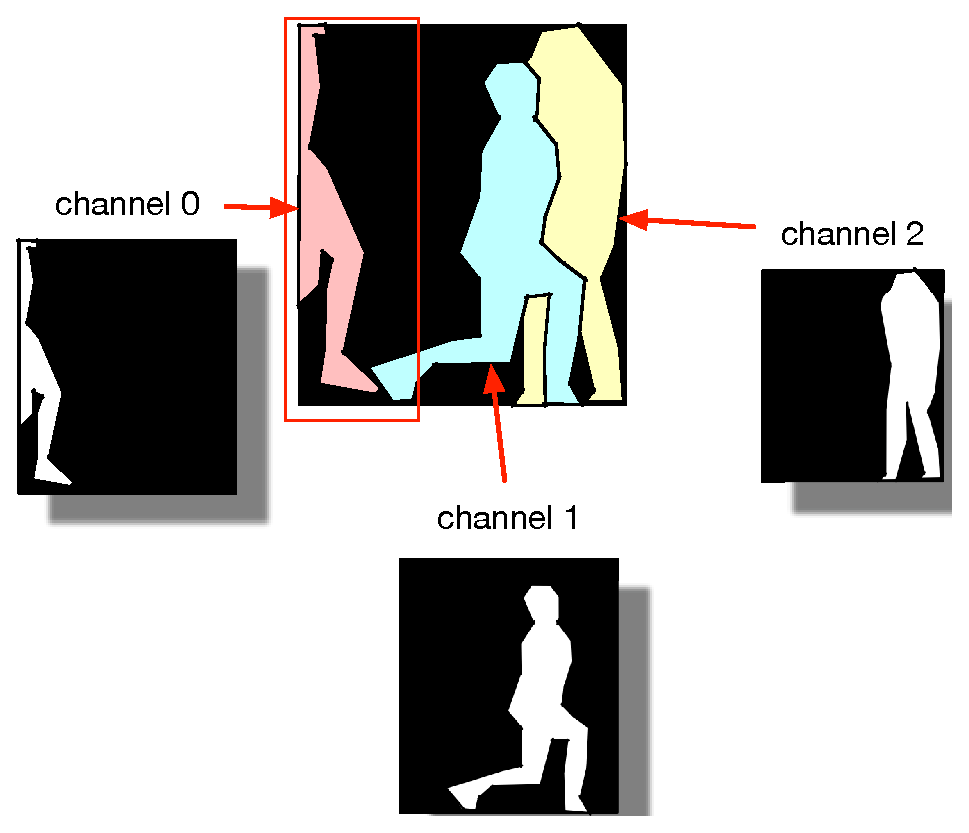
\includegraphics[scale=0.34]{instance_segmentation.eps}
	\caption{Channel-wise instance segmentation}
	\label{fig:chInsSeg}
\end{figure}

\section{本章小结}
